\chapter{方程组}

\begin{introduction}
	\item 预备知识
	\item 数列极限
	\item 函数极限
	\item 连续与间断
\end{introduction}

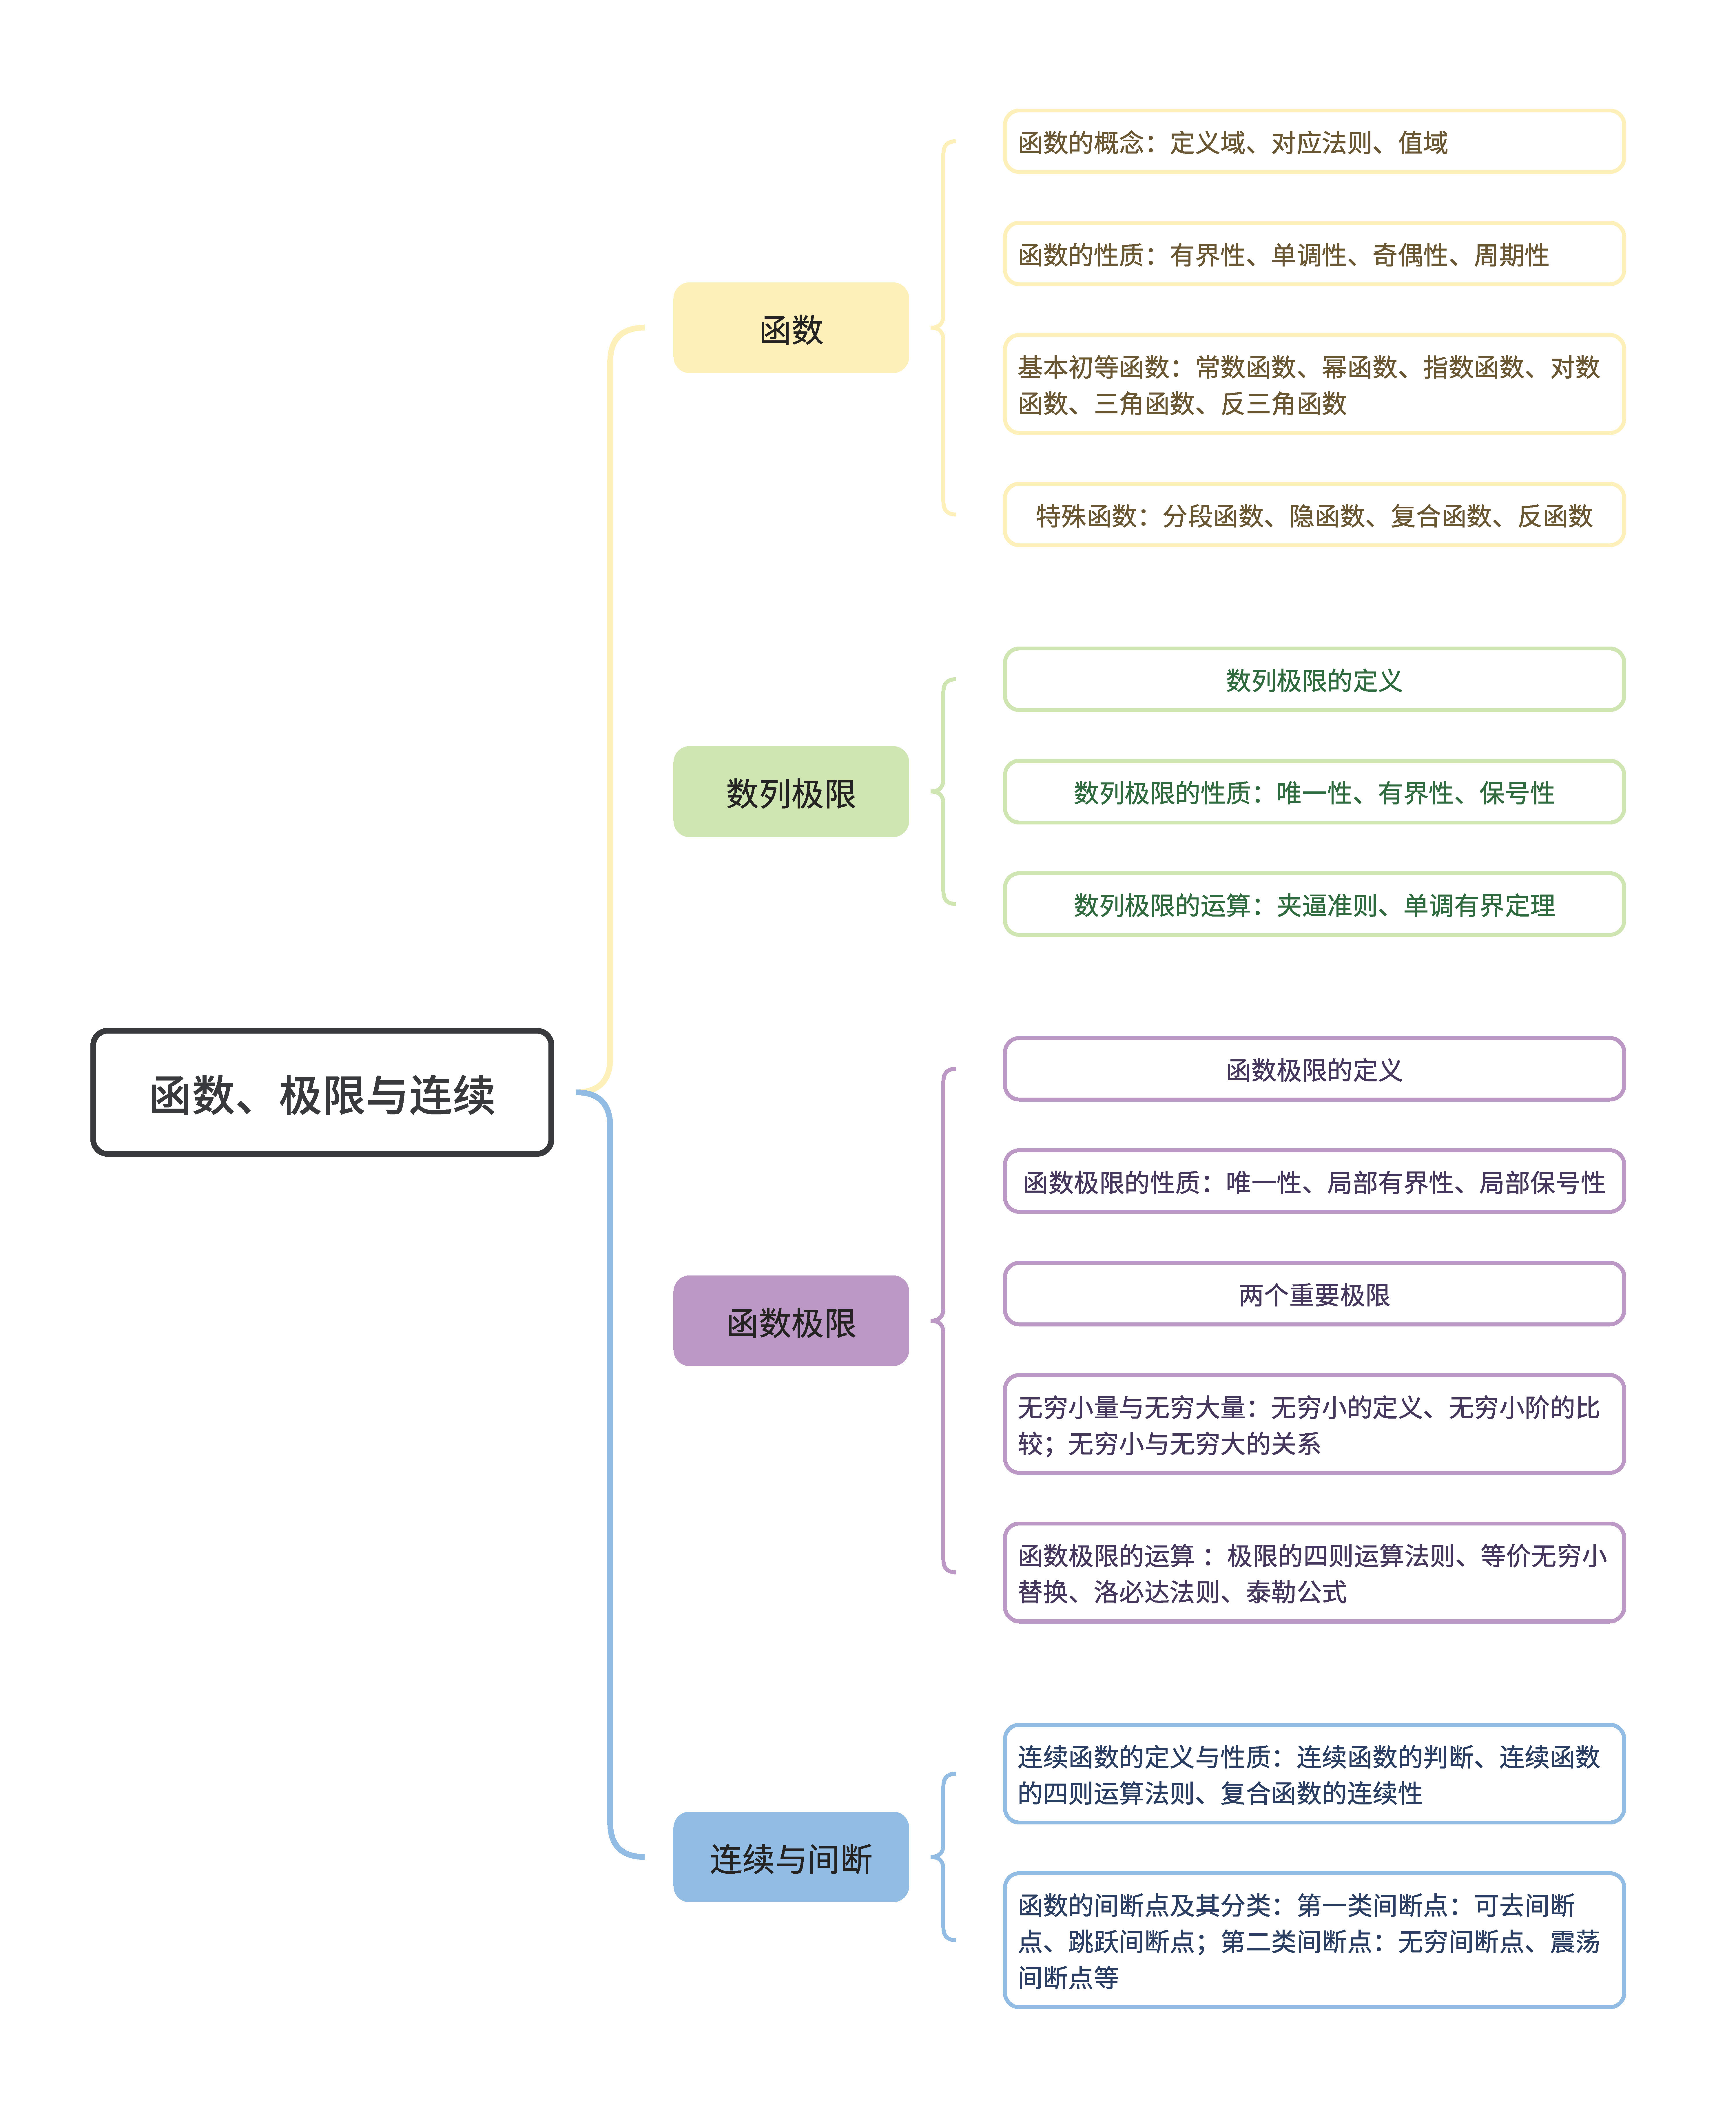
\includegraphics[width=6cm]{figure/chapter/chapter1.jpg}

\section{函数、极限与连续}
\begin{exercise}

设 $P(x)=A(x-1)+B(x-1)^2+C(x-1)^3$ 是函数 $f(x)=x^x-1$ 在点 $x=1$ 处的三阶泰勒多项式，则\fillparen[ ]
	\begin{choices}[columns=5,label-align=center]
		\item 1
		\item 2
		\item 3
		\item 4
		\item 5
	\end{choices}
	
\end{exercise}

\begin{example}	
	设 $P(x)=A(x-1)+B(x-1)^2+C(x-1)^3$ 是函数 $f(x)=x^x-1$ 在点 $x=1$ 处的三阶泰勒多项式，则\fillparen[ ]
	\begin{choices}[columns=5,label-align=center]
		\item 1
		\item 2
		\item 3
		\item 4
		\item 5
	\end{choices}
	
\end{example}




